% HEADER
\documentclass[class=article, crop=false]{standalone}
\usepackage{00_Preamble/frr_preamble}

% Packages
\usepackage{titlesec}
\usepackage{hyperref}
\usepackage{float}
\usepackage{graphics}
\usepackage{placeins}
\usepackage{adjustbox}

\renewcommand{\arraystretch}{1}
% END HEADER

\begin{document}
	\subsection{Concept Development}
	\label{subsec:concept_development}
	\subsubsection{Design Philosophy}
	An entirely new rover design had to be developed for the team’s first year competing in the RMC. With so many design parameters, it was essential to identify a few key design considerations to focus the brainstorming and concept development process. The team focused on maximizing gravel collection, optimizing all systems for autonomy, and simplifying the fabrication process.
	
	
Optimizing gravel collection was the highest priority. The rover must excavate gravel to fulfill its main purpose. Weight and power requirements were considered as well, but it was decided to provide the weight and power necessary to reach the desired goal of excavating 40 kg of gravel. Autonomy was also essential to the design, as the success of future manned missions to Mars depends on reliable autonomous robotic aid. All systems were optimized to be fully autonomous, with the implementation of SLAM and path planning algorithms a major priority for the programming team. With only a nine month project timeline, it was important to eliminate complexity with the use of off-the-shelf components. Stock parts increase system reliability since they are manufactured to higher tolerances than possible in-house. Fabricating custom parts increases lead time and halts progress on dependent systems. However, the team decided to fabricate custom parts when needed so to not limit the design process.

	\subsubsection{System Requirements}
	The robot was designed according to the system requirements defined by NASA as well as requirements defined by Vanderbilt Robotics. The system requirements were classified by the following categories: functional, performance, and budget. All of the requirements are presented in Tables \ref{table:nasa_requirements} and  \ref{table:vur_requirements} below.
	%NASA SYSTEM REQUIREMENTS
	\FloatBarrier
	\begin{table}[h]
	\centering
	\begin{tabular}{ | m{38em} | } 
 	\hline
 		\textbf{Functional} \\ 
 		\hline
 		The robot shall fit within dimensions of 0.75 m x 1.5 m x 0.75 m at the beginning of the competition run. \\ 
 		\hline
 		The robot shall weigh no more than 80 kg. \\ 
 		\hline
 		The robot must report the amount of energy it has consumed since its power-on. \\
 		\hline
 		\textbf{Performance} \\ 
 		\hline
 		The robot must be able to capable of collecting and depositing a minimum of 1 kg of icy simulant within 10 minutes. \\
 		\hline
 		The robot shall be designed to minimize dust kickup and have a dust tolerant design.  \\
 		\hline
 		The robot shall be able to function fully autonomously and failover to human control in the case of an error. \\
 		\hline
 		\textbf{Budget} \\
 		\hline
		The robot design shall be complete and verified by May 1, 2018 \\
 	\hline
	\end{tabular}
	\caption{NASA Defined System Requirements}
		\label{table:nasa_requirements}
	\end{table}
	\FloatBarrier
	
	%VUR SYSTEM REQUIREMENTS
	\FloatBarrier
	\begin{table}[h]
	\centering
	\begin{tabular}{ | m{38em} | } 
 	\hline
 		\textbf{Functional} \\ 
 		\hline
 		The robot must be capable of elevating the collected simulant a minimum of 3 inches above the height of the collector bin. \\ 
 		\hline
 		\textbf{Performance} \\ 
 		\hline
 		The robot must be able to capable of collecting and depositing a minimum of 10 kg of icy simulant within 10 minutes. \\
 		\hline
 		\textbf{Budget} \\
 		\hline
		The project cost for development of the robot shall cost no more than \$8000. \\

 	\hline
 		
	\end{tabular}
	\caption{Vanderbilt Robotics Defined System Requirements}
		\label{table:vur_requirements}
	\end{table}
	\FloatBarrier
	
	\subsubsection{System Hierarchy}
	The system hierarchy is depicted in Figure \ref{fig:system_hierarchy}. The frame consists of the structural base of the robot, drive system, and the power distribution systems. The drivetrain was designed for direct drive. Without a suspension system, it was important to be able to control each wheel independently to maneuver obstacles and improve turning capabilities. The excavation system must dig through BP-1 and collect gravel. It was considered making these two independent processes so to not collect BP-1.  The collected gravel The robot controller software handles all input and output for the robot and maintains a state machine for higher-level control of the robot. The autonomy module includes all of the sensors for localizing the robot and mapping the environment. Additionally, all of the software associated with localization, mapping, and path planning are included in the autonomy module. The teleoperation module provides the human robot drivers with control inputs and data readouts. The autonomy module and driver station interface with the robot controller identically.
	
	\FloatBarrier
		\begin{figure}[h]
			\centering
			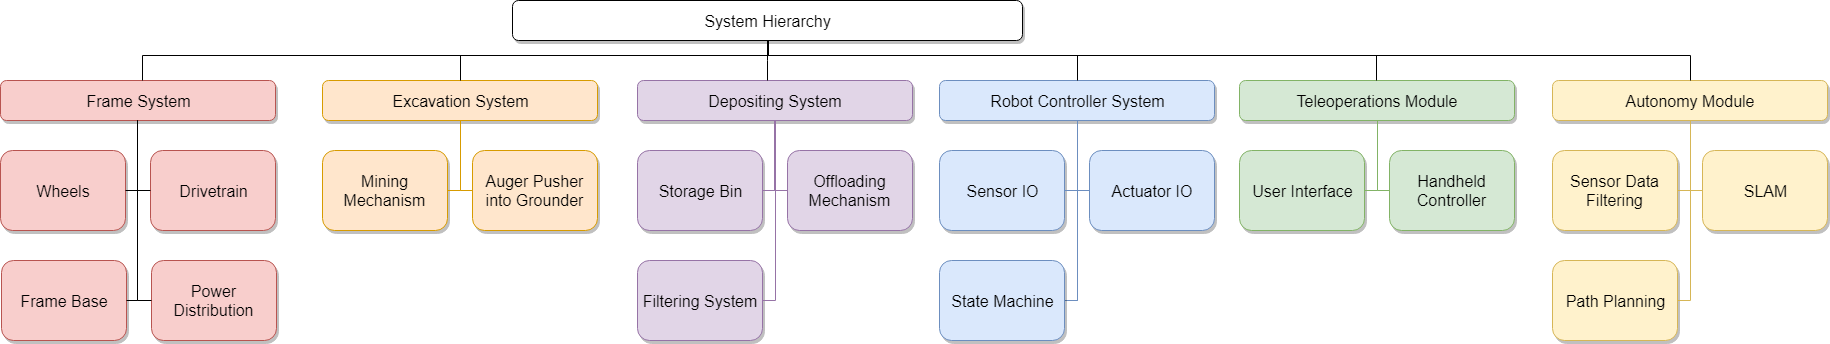
\includegraphics[width=1.0\linewidth]{09_Figures/system_hierarchy.png}
			\caption{Robot System Hierarchy}
			\label{fig:system_hierarchy}
		\end{figure}
		\FloatBarrier
		
	\subsubsection{Concept of Operations}
	The concept of operations are described in Table \ref{table:con_ops} below. The order of operations was derived from the system requirements and key design considerations listed in Section 2.1.2.
	
	%Concept of Operations Table
	\FloatBarrier
	\begin{table}[h]
	\centering
	\begin{tabular}{ | r | l |} 
 	\hline
 		\textbf{Setup}                & 
 		                                Place robot at starting location and set up control station \\ 
 		\hline
 		                              & Power on robot and establish network communication link \\
 		\hline
 		                              & Perform calibration for sensor and control systems on the robot \\
 		\hline\hline
 		\textbf{Competition Start}    & 
 		                                Autonomously scan environment to determine current pose \\
 		\hline
 		                              & Navigate to excavation zone while avoiding obstacles  \\
 		\hline\hline
 		\textbf{Excavation}           &
		                                Mine gravel until section is depleted or storage limit is reached \\
 		\hline\hline
 		\textbf{Post-Competition Run} &
 		                                Record power consumption and turn off the robot \\
 		\hline
 		                              & Clean the robot to remove particulate \\
 		\hline
 		                              & Verify system integrity for next round \\
 		\hline
	\end{tabular}
	\caption{Robot Concept of Operations}
		\label{table:con_ops}
	\end{table}
	\FloatBarrier
	
	\subsubsection{System Requirements Review}
	On October 15, 2017, the executive team members met with the team’s faculty advisor and reviewed the system requirements in preparation for the preliminary design process. The system requirements were confirmed to align with the team’s design philosophy and the competition objectives.The system hierarchy was well modulated to allow for efficient task distribution and system integration. The team agreed that the concept of operations was the correct approach to satisfy both NASA’s requirements and the team-imposed autonomy and gravel collection requirements. The team received approval to proceed to the next design phase.




	
\end{document}
